\documentclass[../../thesis.tex]{subfiles}

\begin{document}

\TODO{Introduce the section, what we think and the philosophy of presenting material in such a way.}

\section{Notation}

\begin{itemize}
    \item Encoder $E$
    \item Decoder $D$
    \item Estimated values are presented with a hat, $\widehat{x}$ for a reconstructed value, $\widehat{f}$ for a trained model etc.
    \item Parameters $\theta$ 
    \item Dataset $X = \{x_i\}_{i=1}^N$  
\end{itemize}

\section{Information theoretic/basic stats used in evaluation}

- maximum entropy distribution

- mutual information

- entropy

- perplexity

- KL-divergence
\url{https://stats.stackexchange.com/questions/188903/intuition-on-the-kullback-leibler-kl-divergence/189758#189758}

- Cross entropy 

- Graphical probabilistic models 
    - Ancestral sampling

- Generative models


\section{Time Series Inference}
- short-time-fourier transform etc.

\section{Neural Network}
An \textit{artificial neural network} or simply \textit{neural network} is a fundamental model in machine learning, and more specifically in \textit{deep learning}. Neural networks are loosely inspired by the way neurons are assembled in the brain. The model can be traced back the year of 1943 when Warren McCulloch and Walter Pitts developed the first artificial neuron \cite{MCCULLOCH199099}, which is considered to be the first neural model invented. It was first set out in the real world by Frank Rosenblatt in 1957 \cite{rosenblatt1957perceptron}. But not until the development of the backpropagation algorithm in its modern form in the 1980's did the model really gain traction. Neural networks have since then been the backbone in the development of machine learning, with an impressive resume of applications. Some of which, if we stretch the definition a bit, include face recognition, beating humans in chess, go and Starcraft, self-driving cars and predicting the structure of proteins. The unreasonable effectiveness of neural networks on a broad range of tasks can in part be explained by the \textit{universal approximation theorem}, proven by Kurt Hornlik in 1989 \cite{HORNIK1989359}, which roughly states that a neural network can approximate any (Borel measurable) function to any desired degree of accuracy. 

\begin{figure}
    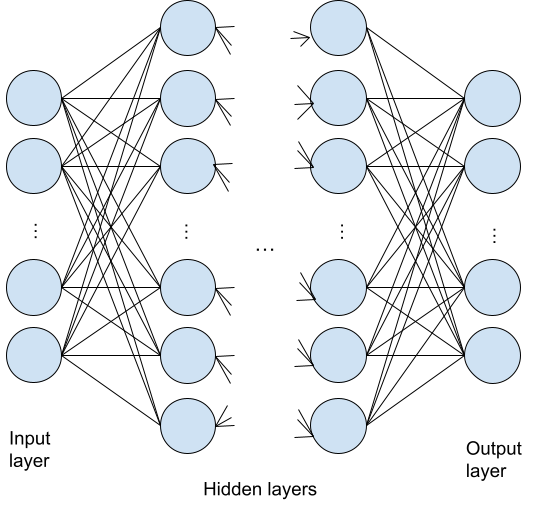
\includegraphics[scale = 0.4]{NeuralNet.png}
    \centering 
    \caption{Illustration of a Neural Network model.}
    \label{fig:NeuralNet}
\end{figure}

A neural network takes in a vector $x \in \mathbb{R}^n$ and builds a nonlinear function $f(x)$ to predict the response $y\in \mathbb{R}^m$. More specifically a neural network maps an input vector $x$ to an output vector $y$ through a series of non-linear functions of linear combinations of the input. This particular structure, presented in figure [fig of nn here] is what distinguishes neural networks from other nonlinear prediction models. The variables $x = [x_1,...,x_n]$ constitutes the units of the \textit{input layer}. The intermediate layers are called the \textit{hidden layers}, and the final mapping to $y$ is called the \textit{output layer}. A neural network is parameterized by a set of \textit{weight} matrices $W_i$ and \textit{bias} vectors $b_i$, together with a specified non-linear \textit{activation function} $\sigma$. Written out a $K$ layered neural network is given by 
\[ 
f(x) = f_K \circ f_{K-1} \circ \ldots \circ f_2 \circ f_1(x),
\]
where 
$$f_i(x) = \sigma(W_ix+b_i), \quad i \in \{1,...,K-1\},$$ 
and $f_K$ is the output layer, with application dependent structure.\\\\ 

The introduction of nonlinearity by the activation function is what enables the model to approximate nonlinear signals and differentiate itself from a linear regression model. Two of the most commonly used activation functions are $\text{Sigmoid}(x) = \tfrac{1}{1+\exp(-x)}$ and $\text{ReLU}(x) = \max(0,x)$, but countless options exists.\newline
The architecture of neural networks, and most specializations thereof, is sequential in nature. They can effectively be described as compositions of some combination of a flavour of matrix multiplication, non-linear transformation and down or upsampling. 

\subsection{Training Neural Networks}

The training of a neural network is the process of finding values for the weight and bias parameters. The general idea governing neural network training is to optimize the parameters based on some distance metric between the predicted values and the target values. This distance metric is referred to as the \textit{loss function}, and common examples of loss functions include mean squared error (MSE) and mean absolute error (MAE). Gradient based methods, such as backpropagation, are usually used to estimate the parameters based on the loss.\newline

The backpropagation algorithm is an efficient application of the Leibniz chain rule for differentiation.\newline

\TODO{Stochastic gradient decent}


For a through introduction to the subject of neural networks and the training thereof we refer to chapter 6 and 8 of \cite{deeplearningbook}.


\section{Convolutional Neural Network}
This section draws heavily on the presentation of convolutional networks in chapter 9 of \cite{deeplearningbook}.\\\\

A convolutional neural network (CNN) is a particular type of neural network that is developed to learn local features in the data. This local feature learning is enabled by the mathematical operation of convolution. In essence a CNN is a neural network where matrix multiplication is switched for convolution at least one of the layers \cite{deeplearningbook}. \newline

Fully connected neural networks have a fundamental drawback in that their computational complexity grows intractably large when the input dimensionality is high. This makes them unsuited for high dimensional data, such as images. Convolutional neural networks directly address this issue via various downsampling techniques. Convolutional neural networks has a rich history and a long track record of success stories. They are inspired by the architecture of visual cortex cells in mammals. Inspired by the discovery of Hubel and Wiesel \cite{https://doi.org/10.1113/jphysiol.1968.sp008455} the neocognitron was proposed in 1980\cite{6313076}. The neocognitron is widely considered the predecessor of convolutional neural networks. In 1989 Yann LeCun et al. introduced the modern framework for CNNs \cite{LeCun1989ConvNet} and demonstrated its effectiveness on the task of hand written digit recognition. Since then CNNs have been an indispensable part of machine learning research, especially in the computer vision domain. For an exposition on the advances on convolutional neural networks and its applications we refer to \cite{gu2017recent}.

\subsection{The convolution operation}

"Convolution leverages three important ideas that can help improve ML systems: sparse interactions, parameter sharing and equivariant representations" \cite{deeplearningbook}.

The convolution operation is an integral transform with extensive applications. It generalizes the notion of a moving weighted average. In mathematics it is ubiquitous because of its relationship with the Fourier transform.\newline

Let $f$ and $g$ be real valued functions, then their convolution is defined as
\begin{equation}
    (f*g)(t) = \int_{-\infty}^{\infty} f(\tau)g(t-\tau) d\tau
\end{equation}

The mathematical nuances of the exact criteria for the above integral to exist is outside the scope of this thesis, and not particularly relevant. But if $f$ and $g$ are integrable (in the Riemann or Lebesgue sense) then the convolution exists. As a rule of thumb, the convolution of $f$ and $g$ is as "smooth" as the smoothest of $f$ and $g$. It is worth mentioning that convolution is commutative, i.e that $f*g = g*f$, which can be seen by a simple change of variables. \newline

As is typical for integral transforms, the function $g$ is referred to as the \textit{kernel}. In the context of convolutional networks the kernel consists of learnable parameters and the function $f$ is the \textit{input}. The output is sometimes referred to as the \textit{feature map} \cite{deeplearningbook}. In machine learning we handle discrete signals, represented as multidimensional arrays. As a result we must employ a discrete variation of the convolution operation. Let $I$ be the input and $K$ be the kernel, both discrete, then their convolution is defined as
\begin{equation}
    (I*K)[n] = \sum_{m=-\infty}^{\infty} I[m]K[n-m].
\end{equation}
In practice $I$ and $K$ typically has finite support, i.e they are zero for large positive and negative arguments, which circumvents any convergence problem.\\\\
Convolutions are naturally defined for higher dimensional functions by component wise extension. For a two dimensional image $I$ and a kernel $K$ we calculate their convolution as 
\begin{equation}
    (I*K)[i,j] = \sum_{n=-\infty}^{\infty}\sum_{m=-\infty}^{\infty} I[n,m]K[i - n,j - m]. 
\end{equation}

\begin{figure}[h]
    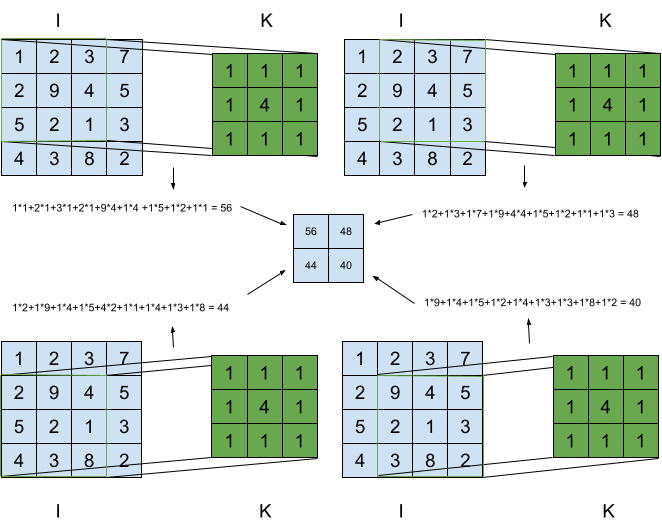
\includegraphics[scale=0.5]{Convolution.png}
    \centering    
    \caption{Illustration of discrete two dimensional convolution}
\end{figure}


- In applications the kernel dimensions are much smaller than the input dimensions. 

- Stride 

- Kernel dim and stride length determines downsample rate (reduction in size). 

- In a convolutional layer the kernel is learned such that the feature map is helpful for the training objective. 


Convolution in machine learning does not always correspond exactly to the mathematical definition of the operation, but rather to cross-correlation. The difference is just a sign flip in the kernel arguments. Operation is no longer commutative, but in practice this does not affect anything as the learned kernel parameters will be equivalent \cite{deeplearningbook}. Machine learning applications are focused on what works, rather than writing proofs. \\\\

\TODO{Concolution in signal processing / image processing in non ml ways. Gaussian kernels, edge detection etc. Provide some hints at why on earth convnets should learn image features.}
\begin{figure}
    \centering
    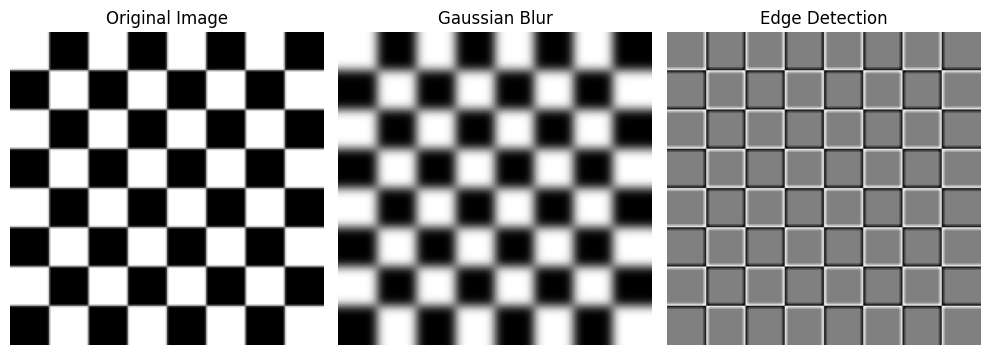
\includegraphics[scale = 0.5]{Kernel_illustration.png}
    \caption{Illustration of discrete convolution applied to images. Image part of Scikit-image data package.}
\end{figure}

\subsection{Pooling}
A pooling operation is applied as a down sample technique on feature maps in CNNs, replacing regions of the output with summary statistics. Two of the most common are max and average pooling, which replaces the region by its maximal or average value respectively. There are two hyperparameters for any pooling operation, the filter size, which determines the region of values to calculate the summary statistic, and stride length, which determines how the filter moves across the feature map. 

\begin{figure}[h]
    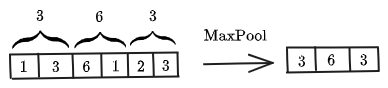
\includegraphics[scale=0.5]{MP_stride2}
    \centering    
    \caption{Max pooling of one dimensional array. Filter size: $2$, stride: $2$.}
\end{figure}
\begin{figure}[h]
    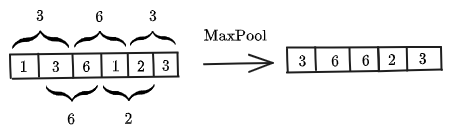
\includegraphics[scale=0.5]{MP_stride1}
    \centering    
    \caption{Max pooling of one dimensional array. Filter size: $2$, stride: $1$.}
\end{figure}

\begin{figure}
    \centering
    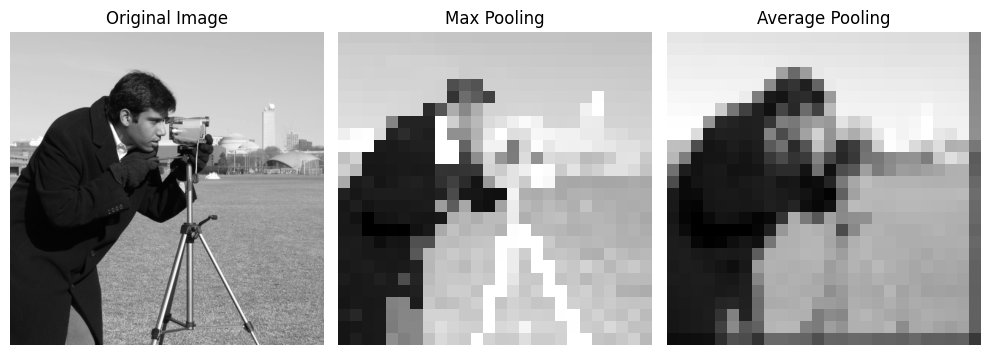
\includegraphics[scale = 0.5]{pooling_illustration.png}
    \caption{Illustration of mean and average pooling applied to images. Original image size is $512\times 512$, pooled images are $26\times26$. Image part of Scikit-image data package.}
\end{figure}

- Pooling assist in making the representations approximately invariant to small distortions of input. 

- Pooling is often essential in handling variable input size.

- 

\subsection{Architecture}
There are a large variety of specific architectures which fall in the category of a CNN, but their basic components are largely the same. They consist of convolutional layers, pooling layers and fully connected layers.\newline

A convolutional layer consists of several kernels used to compute different \textit{feature maps}. Each kernel is applied to the entire input, and the different feature maps are produced by changing kernel. A nonlinear activation function is then applied pointwise to the feature maps.
\TODO{Fig of conv layer}

A pooling layer is typically placed between convolutional layers and work as a stronger downsampler which aims to enforce approximate translation invariance. A pooling operation is applied across each feature map. 
\TODO{Fig of pooling layer}

The fully connected layer is just your typical hidden layer in a neural network, i.e connect every input to every node in the output. 
and is first introduced when the input data has been sufficiently downsampled. The role of these layers is to learn high level reasoning on 
\TODO{Fig of fully connected layer}


\TODO{Fig of CNN}




Convolution: Hidden layer with regular matrix multiplication with weight matrix $W$ is switched out with convolution with kernel matrix $K$.

non-linear activation: Point wise nonlinearity, ReLU, sigmoid etc.

pooling layer: Max, average etc. pooling of feature map.





\subsection{Transposed Convolutional Networks}
Transposed convolution or deconvolution, also known as fractionally-strided convolution is a technique used to reverse the downsampling from convolutions. In essence it is an inpainting or upsampling technique known from digital signal processing. The flexibility of learning data dependent transposed convolutional kernels are. 

\begin{figure}
    \centering
    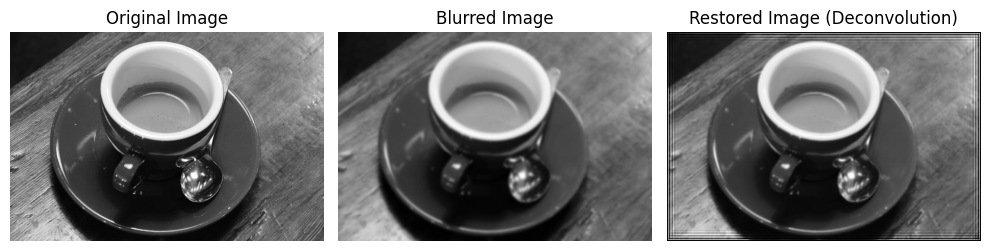
\includegraphics[scale = 0.5]{deconv_illustration.png}
    \caption{Illustration of deconvolution applied to images. Here using Gaussian blur and restoring using the Richardson Lucy algorithm with a Gaussian deconvolution kernel. Image part of Scikit-image data package.}
\end{figure}


% \section{Residual Neural Network}

% Deep neural networks are hard to train. But we want deeper networks as the representations learned in deeper networks tend to be higher level/more abstract \cite{zeiler2013visualizing}. 

% The problem of exploding/vanishing gradients \todo{write about and explain what this is} has been to a large extent been solved by normalized initialization and intermediate normalization layers. This has enabled networks of tens of layers to start converging for SDG with backprop \cite{he2015deep}. \TODO{Rewrite the above in more of my own words}.



% The degeneration problem: 

% The deep residual learning framework was developed to address the degeneration problem.

% \cite{he2015deep}

% \section{Dimension reduction/visualization techniques}

% \subsection{PCA}
% Principle component analysis i a linear dimmension reduction technique which provides the axes of a point cloud 
%  PCA provides a linear projection on the eigenspace of the covariance matrix of the data. 



% \subsection{t-SNE}
% \cite{t-SNE}
% T distributed stochastic neighnourhood encoding.

% \subsection{UMAP}
% \cite{mcinnes2020umap}

% \subsubsection{densMAP}


\section{Representation Learning}

\TODO{Speak on the evaluation metrics for rep learning and the like from \cite{nozawa2022empirical}}
\cite{Rep-rev-persp}
\TODO{Sneak in something about Gödel and Turing in terms of representation. There are many philosophical aspects of this}

\subsection{What is representation learning?}
Representation learning is a term not too easily defined, one reason being the abstraction level. It is helpfull to first consider what is meant by \textit{representation} of information. Lets begin by walking through a familiar and illustrative example. Consider the base ten integer $(4)_{10} = 4$. The number can equivalently (in terms of information content) be expressed, that is represented, in any other base. The particular base we choose depends on our intention with the number. If we want to work with digital electronics, a binary representation ($(4)_{2} = 10$) is very useful, as transistors has two states. When humans do arithmetic, base ten representations of the integers are very natural, as we have ten fingers. A particular representation of information can make a task easier or harder. The information content is unchanged by a change of representation. What is changed is the easiness or difficulty of certain information processing tasks. Representation learning is then the process of learning a certain representation of information. \\\\

Representations are too highly dependent on who, or what, that will process it. An example is time. Humans have developed a standardized system for writing timestamps which works fairly well for us. But, if we want to model time dependent phenomena, say using tabular data, the DateTime representation is of very little help to a tree based model for instance. The reason being that the numerical representation of timestamps close in time is not necessarily close in numerical value. Think of 23:59 to 00:00. A possible solution is to change the representation such that the numerical values actually respect the periodic nature by mapping to the circle. The new representation is then useless for humans, but quite a lot more useful to a computer. \\\\

Anyone who has worked with data science or machine learning has come across feature engineering, and the effect good feature engineering has on a models performance. The same people too knows the level of domain expertise, creativity and time is needed to feature engineer well. One of the intriguing and promising features of neural networks, with its many specializations and architectures, is the ability to learn abstract representations of the data. This is sometimes referred to as automatic feature engineering. \todo{Find som references on higher order features learned in CNNs} In a $N$-layered network $f = f_N\circ ...\circ f_1$, the intermediate value of the data $x$ in some layer $n$ is what is meant by the networks learned feature representations. When we are interested in the representations learned it thus is helpful to dissect a model $f$, notation wise, into a \textit{feature extractor} $h$ and an \textit{output function} \todo{better name??} $g$ such that it can be factored as $f = g \circ h$. Representation learning algorithms typically follow the pattern
\begin{itemize}
    \item Train $f= g \circ h$ on some task, be it supervised, unsupervised etc.
    \item Discard $g$
    \item Use the learned feature extractor $\widehat{h}$ as part of a new model. 
\end{itemize}


The different use cases of $\widehat{h}$ is as stand alone one/few-shot learners (downstream task / frozen protocol) or as initialization of other models (pre-trained / fine-tuning protocol). \newline

When training a neural network of any variation in a supervised fashion, one always get a feature extractor, at no additional cost.  
Unsupervised representation learning loss: reconstruction in AE type, similarity losses in joint embedding networks
\TODO{When mentioning autoencoders, it is a natural spot to talk about compression. "If you can still reconstruct the signal, then you know everything about it in a sense"}


Typically in representation learning algorithms, the output dimension of $\widehat{h}$ is smaller than the input dimension. The idea of compression in representation learning has gotten theoretical and philosophical attention \todo{Information bottleneck, compression}. 


% In more general terms a \textit{feature extractor} is a mapping $h:\mathbb{R}^I \to \mathbb{R}^d$, where $I$ is the input dimension of the model. Typically $d$ is smaller than $I$.\TODO{Something about compression and effective representations}



% In supervised representation learning, the feature extractor $h$ by solving a supervised task.  Examples include $h(x) = f_n\circ ...\circ f_1(x)$ in a NN or CNN.

% One of the advantages of supervised representation learning is that one obtains the feature extractor as a byproduct of supervised learning. 
% \\\\

% Unsupervised, or self-supervised representation learning. The difference form supervised representation learning is that the feature extractor $h$ is learned by an unsupervised objective. 

% Encoder 

\subsection{Why do we care about representation learning?}
\TODO{Rewrite, i have copied to much}
Representation learning is particularly interesting because it provides one way to perform unsupervised and semi-supervised learning. It promises to unlock deep learning for unlabeled datasets. Furthermore it is known that the performance of machine learning methods is heavily dependent on the choice of data representations. Therefore much of actual efforts in deploying machine learning algorithms revolves around constructing good data pipelines and data transformations that results in representations suited for the ML algorithm. Being able to automate such processes, i.e automatic feature engineering, would solve massive problems and ease the use of ML considerably. 


\subsection{What is a good representation?}
\TODO{Talk about the trend of pre-trained models, language representations, tokenization, GPT etc}
\TODO{Rewrite, i have copied to much}
For any representations extracted of a non-invertible function, a downstream task can always be designed (in principle) to based on the lost information, hence achieve arbitrarily bad performance. The concept of universally good representations is therefore ill-defined. There is no free lunch in representation learning either. One must specify a set of predefined \textit{downstream tasks}, and evaluate according to those. The goodness of a representation is determined by how easy it makes the downstream task. Intuitively the quality of the representations are also considered higher if the the representations is able to perform well on several downstream tasks. 


\subsection{How does one evaluate representations?}
As defined in \cite{jing2019selfsupervised} a \textit{pretext task} is a pre-designed task for a network to solve, where the goal is to learn representation. A downstream task is a task used to evaluate the quality of learned representations. In general the downstream task is solved in a supervised manner, using human annotated data.\newline
We let $f = g\circ h$ be a model and train it on a pretext task in order to obtain $\widehat{f} = \widehat{g}\circ \widehat{h}$. As mentioned previously, the quality of learned representations is determined by the performance of the feature extractor $\widehat{h}$ on the downstream task. The standard evaluation protocol is to train a linear head $g_D$ on top of the \textit{frozen} representations in a supervised manner and evaluate this models performance. This is to say that we train  $f_D = g_D\circ \widehat{h}$ by only updating the parameters of the linear model $g_D$, and evaluate $\widehat{f}_D$ on some test set. A common downstream task is classification, where the idea is that good and informative representations should differentiate data in such a way that it is easy to separate them. \newline

\TODO{The role of Visual inspection}


\section{Transformers}

When was it introduced, and by whom?
What lead up to its creation?
Why and where is it now widely used? 


Wiki: A deep learning architecture based on the multi-headed attention mechanism proposed in the 2017 paper "Attention is all you need".

One of the main novelties of the architecture is not relying on recurrence, and instead solely using the attention mechanism to capture dependencies between input and output. As recurrent models are, in computational aspects, inherently sequential, there are major challenges when training as context windows, and sequence lengths become longer. 



\subsection{The attention mechanism}

\TODO{Wait for 3b1b video for context}

\begin{figure}[h]
    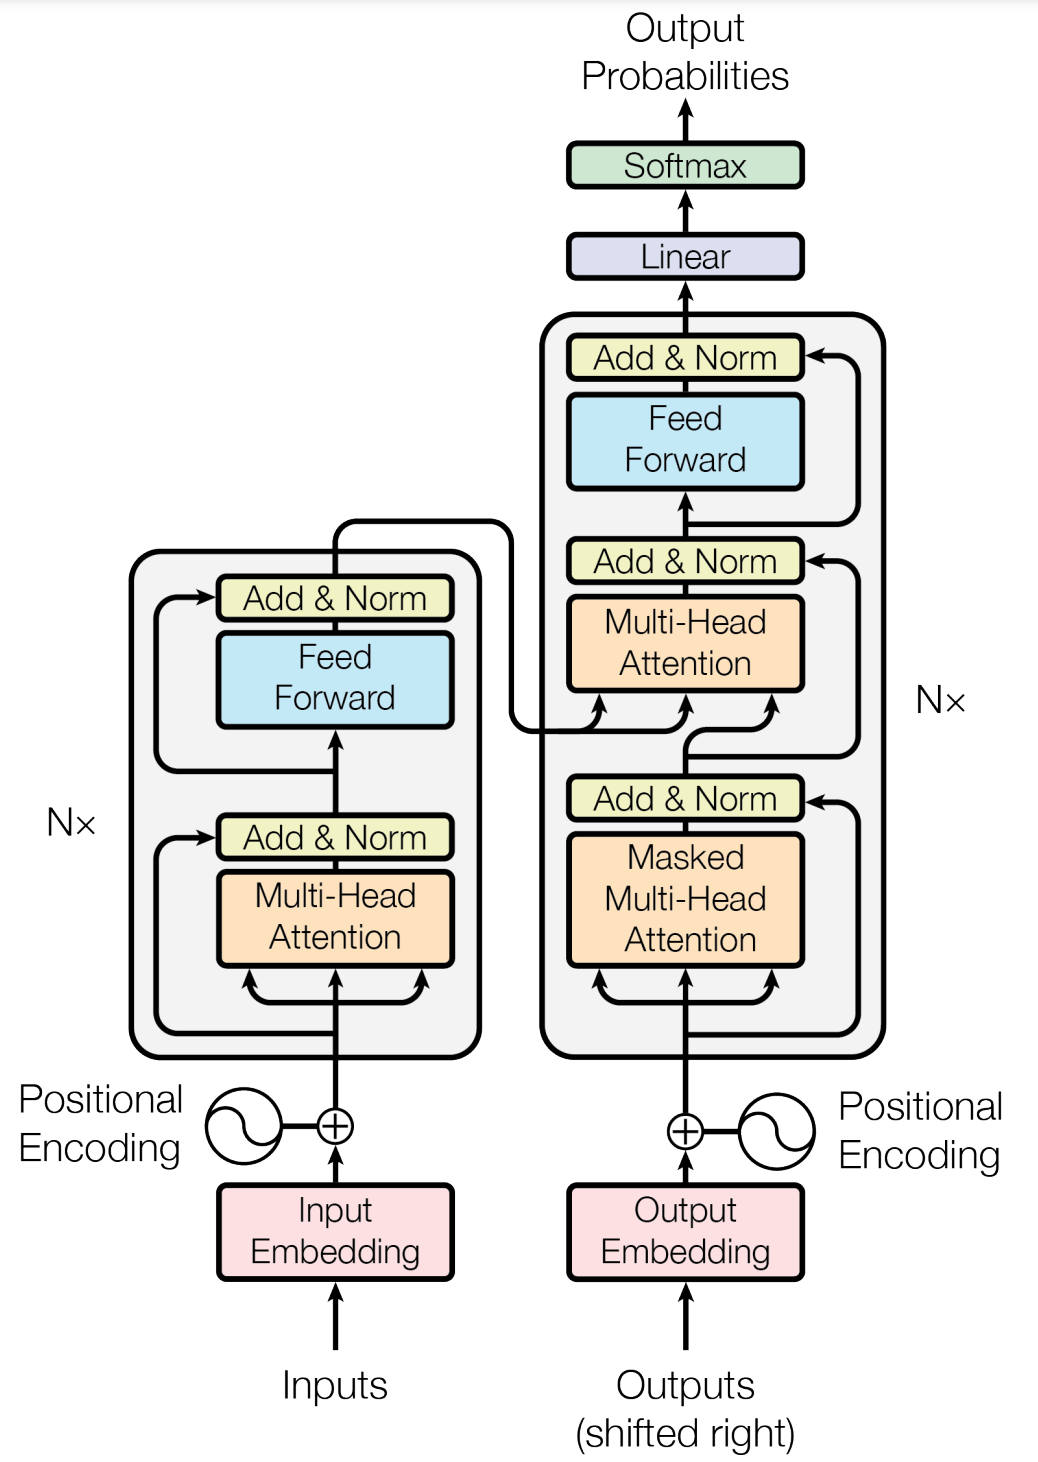
\includegraphics[scale=0.1]{Transformer_architecture}
    \centering    
\end{figure}

\subsection{Architecture}

Tokenizer

Positional encoding


Transformer layer (encoder/decoder)

\subsection{Bi-directional transformer (BERT)}

Unidirectional / 



\section{Self-Supervised learning}

Self-supervised learning (SSL) has had great success in natural language processing and computer vision in recent years. 

Machine learning can be coarsely divided into two classes, supervised and unsupervised learning. 

\subsection{Supervised}
Supervised learning refers to models who learn using labeled data. That is to say for a given input $x$ we already know what the desired output $y$ is during training, and can therefore supervise (update) our models parameters by directly comparing model output and the true value. A bit more formally, for a dataset $X = \{x_i\}_{i=1}^N$ with corresponding human annotated labels $Y = \{y_i\}_{i=1}^N$, the objective of a supervised learning algorithm is to fit $f_\theta$ in such a way that the loss across the data is minimized
\begin{equation}
    \widehat{f}_\theta = \min_\theta \frac{1}{N} \sum_{i=1}^N L(f_\theta(x_i),y_i).
\end{equation}
Common approaches to supervised learning for neural networks is to calculate some distance metric between the predicted value $\widehat{y}$ and the true value $y$ and update parameters by backpropagation.\\\\
The models falling under the supervised learning category are widely deployed and has seen tremendous success. Classical statistical models, as well as support vector machines and decision tree based models are all examples of models in this learning paradigm. The main issue with supervised learning is the need for labeled data, and labeled data is in many ways scarce.

\subsection{Unsupervised}
Unsupervised learning on the other hand refers to models or algorithms who learn exclusively from unlabeled data. That is to say that the models learn intrinsic patterns in the data. Examples of unsupervised learning models are clustering methods as K-means, K Nearest Neighbor and Gaussian mixture models, dimension reduction techniques as PCA/SVD and neural network architectures such as Autoencoders. 


\TODO{Where is it used an why?}
Exploratory data analysis, data visualization, clustering

\TODO{Pros and cons of unsupervised learning}
Unlabeled data is cheap, 

\subsection{Self-supervised}
Self-supervised learning is subcategory of unsupervised learning and refers to model who use the data itself to generate a supervisory signal, rather than external labels as in supervised learning. Even as SSL is considered unsupervised learning, the learning formulation is quite similar to that of supervised learning.\newline

For a dataset $X = \{x_i\}_{i=1}^N$ with \textit{pseudo labels} $P = \{p_i\}_{i=1}^N$ the objective of a self-supervised learning algorithm is to fit $f_\theta$ in such a way that the loss across the data is minimized. In other words find 
\begin{equation}
    \widehat{f}_\theta = \min_\theta \frac{1}{N} \sum_{i=1}^N L(f_\theta(x_i),p_i).
\end{equation}

A pseudo label is an automatically generated label from the data attributes in the pretext task. In joint embedding architectures the pseudo labels are typically some \textit{augmentation} of the original data.


\TODO{Explain why we care:}

A fruitful approach to unsupervised representation learning.\\\\

Randomly initialized networks are difficult to train and requires a lot of time and computational resources. SSL has shown remarkable results when used for pre-training. That is as models for learning network parameters who capture semantics of data, without the need for labels. Pre-training networks enables foundation models, which can be trained for many different tasks in a supervised fashion, called fine-tuning, requiring a lot less resources.

\TODO{Explain where we are now:}
In recent years, especially in computer vision applications, SSL methods have shown incredible promise in representation learning. SSL methods have proven close to, and sometimes surpassing, supervised methods on downstream tasks. \TODO{Find sources backing this up.}


\TODO{What are the different flavours of SSL? }
Autoassociative SSL - Autoencoder type - Essentially try to make composition the identity despite a compression. Usually not considered SSL, but it technically is. 
Contrastive vs non-contrastive
\TODO{What are some of the issues?}

Contrastive: Collapse, where encodes produce uninformative or constant vectors. The different ways of handling collapse. How Variance-Covariance regularization (VCReg) \cite{mialon2024variance} has emerged as a minimal(??) solution. 


\subsubsection{Contrastive}
Contrastive SSL includes both positive and negative samples. The loss function of contrasitive SSL attempts to minimize the distance of positive sample pairs (+,+) and (-,-), and maximize the distance between negative sample pairs (+,-) and (-,+).\\\\

\subsubsection{Non contrastive}

Augmentations for creating different views. The role of augmentations, types etc. Augmentations across modalities. 

\subsubsection{Joint embedding architecture}

Joint embedding architecture: An architecture where two networks are trained to produce similar embeddings for different views of the same data. A popular joint embedding architecture is the siamese network architecture \cite{siamese}, in which the two networks share the same weights. In models with such architecture, the existence of trivial solutions, such as both networks ignoring input and produce identical constant embeddings, is a major issue. This issue is referred to as \textit{collapse} of the model.

\subsubsection{The role of projectors}

\subsection{Masked modelling}
Masked modelling is a conceptually simple self-supervised learning technique for generative models. The idea is to mask or cover a portion of the input data and predict the masked portions. By comparing the prediction against unmasked data the model can learn useful representations without supervision. Since the introduction of masked modelling in natural language processing by \cite{devlin2019bert} it has been the de-facto standard for self-supervised pretraining of language models. BERT introduced masked modeling for language representation learning as means to use bi-directional transformers without enabling each word to "see itself". \newline
\TODO{When did GPT \cite{Radford2018ImprovingLU} use Masked modelling?}

When vision transformers \cite{dosovitskiy2021image} surpassed CNN in 2021\cite{he2015deep}, CV research began to draw inspiration more heavily from \cite{devlin2019bert} and began tokenizing images and pretraining transformers.\newline
Masked image modelling \cite{he2021masked}: Mask image patched directly \newline
Masked visual token modelling \cite{chang2022maskgit}: Tokenize the image and mask tokens. \newline



\TODO{Masking in original domain or tokens. Masking strategies.}

For a thorough survey on masked modelling for SSL in the vision domain we refer to \cite{li2024masked}. 





\section{Vector Quantized Variantional Autoencoder (VQVAE)}
Our model is based on the Vector Quantized Variantional Autoencoder (VQVAE) introduced in \cite{VQVAE}, and includes an Auto-encoder (AE) branch. Therefore it is natural to dive into the models. We first start with introducing auto-encoders, then present the variational variation VAE before presenting VQVAE. 

\subsection{Autoencoder (AE)}

Consists of two neural networks, an encoder $E$ and decoder $D$. They can be seen as maps between spaces $X$ and $Z$, where we refer to $X$ as the data space and $Z$ as the latent space. 
\TODO{Architecture figure}
\begin{equation}
    X \xrightarrow{E} Z \xrightarrow{D} X 
\end{equation}

The autoencoder is trained in such a way that the composition of encoder and decoder is approximate to the identity. Typically, if the model is to learn interesting, the dimension of the latent space is lower that that of the data space. Encoder and decoder then compresses and decompresses the data and learns efficient \textit{latent representations}. 
\TODO{Information bottleneck}
\TODO{Issues with latent representations and the need for regularization}

\subsection{Variational Autoencoder (VAE)}
Variational Autoencoders (VAE) were introduced in \cite{kingma2022autoencoding} and is a variational Bayes approach to approximate inference and learning with directed probabilistic models. The architecture of VAE is similar to AE, but the mathematical formulation is quite different. For context variational inference is a technique in statistics used to approximate complex distributions by looking for the closest approximation within a simple, but flexible, parameter family. \newline 

\TODO{Intractabilities, why an how?}

We assume that the dataset $X = \{x_i\}_{i=1}^{N}$ consists of iid samples from a random variable $\mathbf{x}$. In the VAE framework we further assume that the data is generated by some unobservable random process. This is to say that we assume there is a random variable $\mathbf{z}$ such that $x_i \sim p_{\theta^*}(x|z_i)$, where $z_i \sim p_{\theta^*}(z)$. The distribution $p_{\theta^*}(z)$ is referred to at the true prior and $p_{\theta^*}(x|z_i)$ as the true likelihood. As $\mathbf{z}$ is unobservable and the true distributions are unknown, one has to assume their form. In general the prior and likelihood are assumed to be from parametric families $p_{\theta}(z)$ and $p_{\theta}(x|z)$. As with any model where one wishes to employ gradient based learning, the distributions are assumed to be differentiable almost everywhere, both with respect to their parameters and argument.\newline
\begin{figure}[h]
    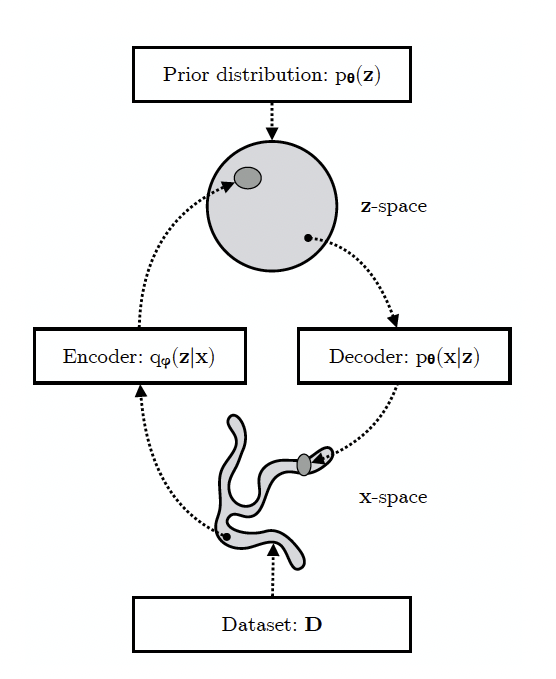
\includegraphics[scale=0.3]{VAE}
    \centering  
    \caption{\cite{VAE}, need to ask for permission or make own}  
\end{figure}

VAEs have two components to their architecture. The first is a probabilistic encoder, often called the inference model, $q_\phi(z|x)$ which approximates the true posterior. Secondly a probabilistic decoder, often called the generative model $p_\theta(x|z)$, which approximates the likelihood. These models are typically parameterized by some type of neural network, and in that case $\phi$ and $\theta$ are the weights and biases of the two networks. Given a datapoint $x_i$ the probabilistic encoder provides a distribution over the possible values of the latent variable $\mathbf{z}$. Similarly, given a latent representation $z_i$ the probabilistic decoder produces a distribution over the possible corresponding values of $\mathbf{x}$. \newline

The probabilistic part of the encoder and decoder is the sampling part. The output for a given $x$ or $z$ is a distribution, and for the same input the same output distribution is calculated (as long as the network parameters are frozen). Actually $x$ and $z$ are mapped to the parameters of a distribution, which uniquely determines the distribution in a particular family.\newline

The most common situation is to assume 
\begin{itemize}
    \item Prior $p_\theta(z)\sim N(0,I)$
    \item Likelihood $p_\theta(x|z)\sim N(D(z), I)$ ??? Is this true? 
    \item Variational posterior $q_\phi(z|x)\sim N(E(x)) = N(\mu_x, \Sigma_x)$
\end{itemize}

In a VAE the encoder maps datapoints to parameters of the variational distribution, i.e the approximate posterior $q$. $x \mapsto E(x) = (\mu_x, \Sigma_x)$. A latent representation $z$ is then sampled from $q$, which constitutes the random part of the algorithm. The decoder maps $z$ to the expected value of the likelihood $p(x|z)$. $z_i \mapsto D(z_i)$. \newline

There are several reasons for choosing this family, one being that the Gaussian distribution a scale-location family. This enables us to circumvent the problematic random component in the VAE when using gradient based learning. As described above we sample $z\sim N(\mu_x,\Sigma_x)$ where $E(x) = (\mu_x,\Sigma_x)$. We can equivalently sample from $N(\mu_x,\Sigma_x)$ by reparameterization using the location-scale property. This means to introduce an auxillary variable $\epsilon \sim N(0,I)$ and rewriting $z = \mu_x + L_x\epsilon $, where $L_x$ is the Cholesky decomposition of $\Sigma_x$. This factors the random part out of path of gradient flow.\newline
\TODO{Illustration of computational flow/gradient flow.}



\subsubsection{Training objective}

As with other variational methods, VAEs are optimized with respect to the \textit{evidence lower bound} or ELBO for short. Let $X$ and $Z$ be two jointly distributed variables, with distribution $p_\theta$. Then for any distribution $q_\phi$ the ELBO is defined as

\begin{equation}
    \label{eq:ELBO}
    \loss_{\theta,\phi}(x) 
    = \mathbb{E}_{q_\phi(z|x)} \log \left( \frac{p_\theta(x,z)}{q_\phi(z|x)}\right)
\end{equation}
The ELBO can be reformulated in terms of the marginal likelihood and KL divergence of the variational to the true posterior.
\begin{equation}
    \begin{aligned}
        \label{eq:ELBO_loglik}
        \loss_{\theta,\phi}(x) 
        &=  \mathbb{E}_{q_\phi(z|x)} \log \left( p_\theta(x)\right) + \mathbb{E}_{q_\phi(z|x)} \log \left( \frac{p_\theta(z|x)}{q_\phi(z|x)}\right) \\
        &= \log \left( p_\theta(x)\right) - \textrm{KL}(q_\phi(z|x)|| p_\theta(z|x)).
    \end{aligned}
\end{equation}
Due to the non-negativity of the KL-divergence, we see that the ELBO bounds the marginal log likelihood of the data from below. By maximizing the ELBO with respect to the model parameters $\phi$ and $\theta$ one simultaneously maximizes the marginal likelihood, which improves the generative model, as well as reducing the KL-divergence of the approximate to the true posterior, which improves the inference model \cite{VAE}.\newline
An alternative reformulation gives a more evident connection to Auto-encoders, with a the prior acting as a regularizer on the posterior 
\begin{equation}
    \begin{aligned}
        \label{eq:ELBO_AE}
        \loss_{\theta,\phi}(x) 
        &=  \mathbb{E}_{q_\phi(z|x)} \log \left( p_\theta(x|z)\right) - \mathbb{E}_{q_\phi(z|x)} \log \left( \frac{q_\theta(z|x)}{p_\phi(z)}\right) \\
        &= \underbrace{\mathbb{E}_{q_\phi(z|x)} \log \left( p_\theta(x|z)\right)}_{\text{Expected reconstruction log likelihood}} - \underbrace{\textrm{KL}(q_\phi(z|x)|| p_\theta(z))}_{\text{Regularizer}}.
    \end{aligned}
\end{equation}
As the $p_\theta(x|z)$ is typically assumed to be Gaussian we have

\begin{equation}
    \log p_\theta(x|z) = -\frac12 \left[k\log(2\pi)+ (x-D(z))^T(x-D(z))\right],
\end{equation}
which is equivalent, as an optimization objective of $D(z)$, to $||x-D(z)||_2^2$. Consequently the likelihood in the loss is implemented as the MSE of the input $x$ and the output $D(z)$.

\subsubsection{Generative model}
The role of the prior in a VAE is two fold. Firstly as a regularizing constraint for the posterior during training, and secondly as a way of obtaining new samples $x$ via ancestral sampling. Ancestral sampling refers to $\z$ being the parent node of $\x$ in the VAE, and that we can generate samples $x$ by drawing a sample $z\sim p(z)$ and decode $D(z)$. 


% This is known as \textit{prior predictive sampling}. 
% The other option is to use \textit{posterior predictive sampling} by using a datapoint $x_i$ to obtain a posterior distribution $q(z|x_i)$, sample a latent representation $z_i$ and then obtain $p(x|z_i)$. From this likelihood we can sample implicitly conditional on $x_i$. 



\TODO{Speak on limitations of VAE before introducing VQVAE}
Variational autoencoders has the issue of collapsing. Variance issues.


\subsection{Vector Quantization (VQ)}
Dictionary learning model \cite{Gray1984VQ}

\subsection{VQVAE}
The Vector Quantized Variational AutoEncoder (VQVAE) was first introduced in \cite{VQVAE} and presented a new way of training VAEs with discrete latent variables. It is the first discrete VAE model which has similar performance to the continuous variant. VQVAE was developed to learn useful discrete representations for generation. This is enforced by more flexible distributional assumptions, as they say "Our model, the Vector Quantised-
Variational AutoEncoder (VQ-VAE), differs from VAEs in two key ways: the
encoder network outputs discrete, rather than continuous, codes; and the prior
is learnt rather than static."-\cite{VQVAE}. 
\newline
The overall architecture of VQVAE consists of an encoder and decoder as before, together with a \textit{codebook} which is used in the quantization process. The codebook, also referred to as the latent embedding space, $\mathcal{Z} = \{z_k\}_{i=1}^K$ is consists of $K$ latent vectors with dimensionality $D$. It can be considered a lookup table of vectors that are used for vector quantization (VQ). The output of the encoder $E(x)$ is quantized by the means of nearest neighbor lookup
\begin{equation}
    z_q = \argmin_{z_k\in\mathcal{Z}} ||E(x)-z_k||.
\end{equation}
In the original article \cite{VQVAE} they propose to separately learn the prior distribution, after the encoder, decoder and codebook is learned. During the initial training the prior is assumed to be uniform, which poses no constraint on the posterior learning. \newline

In contrast to VAEs the posterior is assumed to be categorical, as opposed to normal and the probabilities are defined as
\begin{equation}
    p(z=k | x) = 
    \begin{cases} 
        1 \quad \text{for }k = \argmin_j||E(x) - z_j||_2 \\
        0 \quad \text{otherwise}
    \end{cases},
\end{equation}
Sampling from the posterior amounts to quantizing the output of the encoder, as it is deterministic. \newline

VQVAE can be viewed as a VAE, hence we can bound the marginal likelihood with the ELBO \ref{eq:ELBO_AE}. As the variational posterior is deterministic and the prior (during training) is uniform over $\{1,...,K\}$ we get that the regularizing term

\begin{equation}
    \begin{aligned}
        \KL(q(z|x)||p(z)) &= \sum_{z}  q(z|x) \log \left(\frac{q(z|x)}{p(z)}\right) \\
                           &= q(z=k|x) \log \left(\frac{q(z=k|x)}{p(z=k)}\right) \text{, $q$ is deterministic}\\
                           &= \log \left(\frac{1}{1/K}\right) \text{, uniform prior}\\
                           &= \log(K), 
    \end{aligned}
\end{equation}
is constant. Consequently the ELBO reduces to the reconstruction term only. \newline

\TODO{What do we gain by having a flexible posterior and a non-informative prior during training? The advantages for generative modelling to have a learnable prior? VAEs are traditionally quite bad when it comes to generative quality (sharpness). The flexibility of VQVAE seems to set the stage for better sample generation.}

\TODO{Can think of the codes as the modes of a mixture of Gaussians, and instead of sampling from the mixtrure you just choose the closest mode.}

\subsubsection{Prior Learning}
During the initial training the prior is as mentioned constant and uniform. After training an autoregressive prior is fit on $z$ so we can sample $x$ via ancestral sampling, i.e sample $z \sim p(z)$ and decode $D(z) = x$. The choice of prior model depends on the particular application and in VQVAE PixelCNN \cite{oord2016pixel} was used for image, while WaveNet \cite{oord2016wavenet} was used for audio. More recently in TimeVQVAE \cite{TimeVQVAE} utilized a bidirectional transformer \cite{chang2022maskgit} for prior learning in the time series domain. 

\subsubsection{Loss funciton}
As we want to do gradient based learning, and the quantization process is quite far off from being continuous, measures has to be taken. The output of the encoder and the input of the decoder has the same dimension, which opens the possibility of simply copying the gradients from the decoder input to the decoder output. This is referred to as the \textit{straight through estimator}.\newline

The loss function consists of three parts, the reconstruction loss, VQ loss and commitment loss. We already mentioned that the ELBO objective reduced to the reconstruction term only. In order to learn the codebook one uses the VQ loss, which is the euclidean distance between the encoder output and the quantized output. The final part of the loss is the commitment loss, which is introduced to keep the distance between embedding vectors (or codes) from growing arbitrarily large. To summarize the total loss is given by

    \begin{equation}        
        \begin{aligned}
            \loss_{\text{Recon}} &= ||x - \widehat{x}||_2^2\\
            \loss_{\text{VQ}} &= ||sg(z) - z_q||_2^2 +\beta||z - sg(z_q)||_2^2\\
            \loss_{\text{VQ-VAE}} &= \loss_{\text{VQ}} + \loss_{\text{Recon}}
        \end{aligned}
    \end{equation}

where $\beta$ is a tuning parameter typically set to be $0.25$ and $sg()$ is the stopgradient operation, defined to be the identity with zero partial derivatives. \newline

To illustrate the need for commitment loss and what it does consider a model where the data is either $0$ or $1$ and we initialize the codebook with $\mathcal{Z} = \{-1,1\}$.  The range of the encoder is $\R$ and $E(x)$ is quantized to $-1$ if its negative and $1$ if its positive. Assume that the encoder and decoder will try to differentiate between the two classes by pushing $E(0)$ and $E(1)$ away from each other. As the reconstruction loss only affects the encoder and decoder, and the VQ loss only affect the codebook, we get that when the encoder and decoder parameter trains faster than the codebook, then the distance between the encodings and the codewords will steadily increase and the VQ loss diverge. \newline 

\begin{figure}[h]
    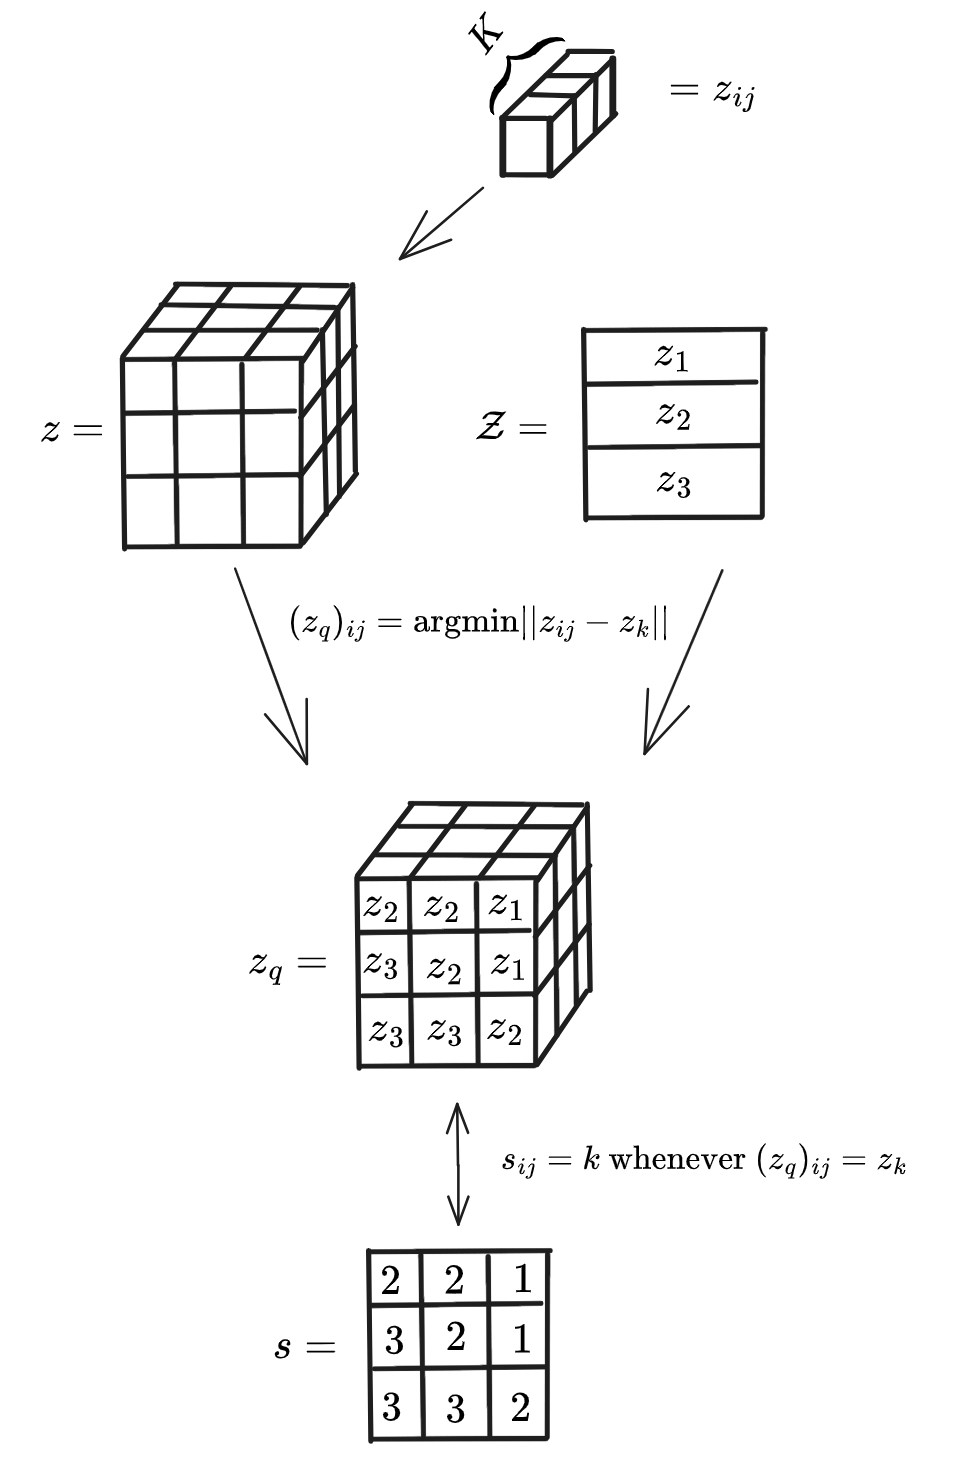
\includegraphics[scale=0.5]{quantization}
    \centering    
\end{figure}

\subsubsection{Orthogonal regularization loss}

There has been several attempts to improve vector quantization. In \cite{shin2023exploration} they advocate for learning orthogonal/decorated codewords. 
% \TODO{Reference https://github.com/lucidrains/vector-quantize-pytorch some way.}



\section{Evaluation metrics}

\subsection{Tokenization model}

The tokenization model, as we are interested in representation learning, is evaluated on two metrics. Firstly, and most importantly its ability to reconstruct the input data once compressed into latent space. In essence the latent representation encodes "everything" (important information is preserved) about the original data if the model is able to reconstruct well. Secondly we evaluate linear classifiers on the latent representations, which provides good results if the model learns discriminative features of the different classes and produces an approximately linear separable space. Finally, as the tokenization model is a part of the generative model, the ultimate evaluation metric is the corresponding evaluation of the generative model. 

\subsubsection{Reconstruction}


\subsubsection{Downstream Classification}

SVM, KNN. The difference in inductive bias for the two classifiers. 


\begin{figure}[h]
    \label{fig:ClassifierComparrison}
    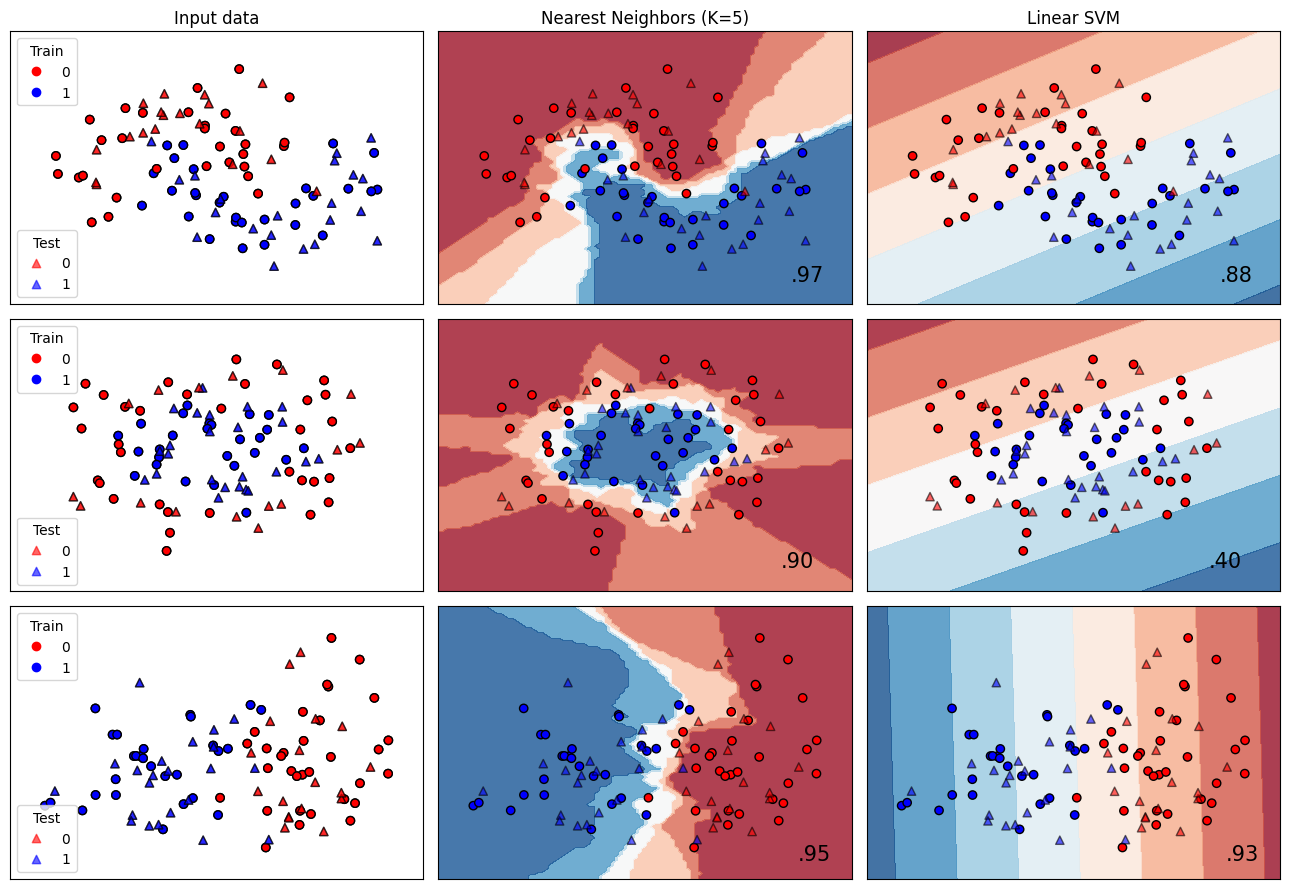
\includegraphics[scale = 0.4]{ClassifierComparrison.png}
    \centering
    \caption{Modified example taken from \url{https://scikit-learn.org/stable/auto_examples/classification/plot_classifier_comparison.html}.}
\end{figure}

\subsection{Generative model}
Good evaluation protocols for generative models are hard to come by, and the hunt for such is an active area of research. There are data modalities for which such evaluation metrics have more established standards than others. Most notably in the computer vision domain there is a benchmark dataset (ImageNet) and classifier (Inception v3). \newline

The typical sanity check for generative models is human visual inspection. In development of generative evaluation metrics how well a proposed metric correlates with quality determined by visual inspection. Most people know what cats and dogs look like and can recognize features even in crudely generated images \todo{lik til artikkel som har dårlig genererte bilder}. In contrast, many time series dataset measure quantities and signals for which the untrained eye has no idea of determining the quality. This is one of the obstacles in TSG, and the evaluation of the evaluation metrics for TSG. \newline 

We mainly consider three evaluation metrics in this thesis, following \cite{TimeVQVAE}. Common for all is the dependency on a external classification model. \textit{Inception Score} (IS), \textit{Fréchet Inception Distance} (FID) and \textit{Classification Accuracy Score} (CAS).
IS measures quality of synthetic samples using the entropy of the label distribution and the evenness in prediction across labels \todo{This sencence is a copy from TimeVQVAE, rewrite or cite. I think it is good.}. The \textit{Fréchet Inception Distance} measures a distance between the generative and ground truth distribution. Finally the \textit{Classification Accuracy Score} measures the quality of the class-conditionally generated samples by training a classifier on synthetic and testing on real data.

Common for all the evaluation metrics is the reliance on a pre-trained classification model. In contrast to computer vision there is no widely adopted classification model for time series, but in \cite{wang2016time} a fully convolutional network (FCN) was presented as a proposed baseline classification model for time series. As their model is not available we use the open source FCN trained on the UCR Archive presented in \cite{TimeVQVAE} for our evaluations. \newline


According to \cite{TimeVQVAE} the most common evaluation protocols in the TSG literature is PCA and t-SNE analyses on time series to visually see similarities of two distributions. The major limitations of this is that the visual inspections cannot be reduced to a single score, which makes objective comparison difficult. \newline


FID score measures difference in the distribution of representations of time series. The representations capture high level semantics of the time series and analyses of these representations can provide greater insights to the realism of generated samples. \newline





\subsubsection{Visual Inspection}

Issues with visual inspection of time series data, compared to modalities as image and audio, is that humans are naturally quite good classifiers of image and audio.


\subsubsection{Inception Score (IS)}
Inception Score (IS) was first introduced in \cite{salimans2016improved} as an automatic evaluation method of synthetic samples.\newline
The Inception Score works by applying a classifier to every generated sample to get the conditional label distribution $p(y|x)$. Samples containing meaningful "objects" should have low entropy, i.e be certain of the label. In addition we expect a good model to generate varied samples, so the marginal $\int p(y|x = G(z))dz$ should have high entropy. Here $G$ is our generative model and $z$ the latent variable. On this basis, the Inception Score is defined as 

\begin{equation}
    \label{IS}
    {\text{IS}}(\theta) = \exp\left( \mathbb{E}(D_{\text{KL}}(p_\theta(y|\mathbf{x}) || p_\theta(y))) \right).
\end{equation}

In contrast to computer vision there is no widely adopted classification model for Time Series. In \cite{wang2016time} a fully convolutional network (FCN) was presented as a proposed baseline classification model, and we use the open source FCN trained on the UCR Archive presented in \cite{TimeVQVAE} for our evaluations. \newline

Let $X_{\text{gen}} = \{x_{i,\text{gen}}\}_{i=1}^N$ be a set of generated samples. We use the apply a SoftMax layer to pretrained FCN representations to obtain an estimate of the conditional label distribution as follows
\[
    x_{i,\text{gen}} \xrightarrow{\mathrm{FCN} + \mathrm{SoftMax}} p(y |x_{i,\text{gen}}).
\]
The marginal label distribution is obtained by averaging across all the synthetic data as follows

\[
    p(y) = \frac{1}{N} \sum_{i=1}^N p(y |x_{i,\text{gen}}).
\]

Issues with IS \cite{barratt2018note} (Use different network, for image classification).  Important to report different metrics that indicate that the model has not overfitted. 
Also issues with IS \cite{borji2021pros}.\newline

\subsubsection{Fréchet Inception Distance (FID)}
As an attempt to improve on IS \cite{heusel2018gans} introduced the Fréchet Inception Distance (FID). Since then FID has been the standard for assessing generative models \cite{borji2021pros}.\newline
The primary concern with IS is, as mentioned earlier, that it does not use any statistics of real world samples to compare with the statistics of the generated samples. In contrast FID relates the synthetic sample to the real world samle via the \textit{Fréchet distance}. For any two probability distributions, $f,g$ over $\R^n$, with finite mean and variances, their  distance is defined as 
\begin{equation}
    \begin{aligned}
        d_F(f,g) &= \left(\inf_{\gamma \in \Gamma(f,g)} \int_{\R^n\times\R^n}||x-y||_2^2d\gamma(x,y) \right)^{\frac{1}{2}}\\\\
            &= \left(\inf_{\gamma \in \Gamma(f,g)} \E_{(x,y)\sim \gamma} ||x-y||_2^2\right)^{\frac{1}{2}},
    \end{aligned}
\end{equation}
where $\Gamma(f,g)$ is the set of all \textit{couplings} of $f$ and $g$. The Fréchet distance is a special case of the Wasserstein metric and will in literature be referred to as such.\newline 

In \cite{DOWSON1982450} it was shown that for two Gaussian distributions the Fréchet distance is explicitly solvable as

\begin{equation}
    \label{eq:FID Gaussian}
    d(\N(\mu,\Sigma),\N(\mu',\Sigma'))^2 = ||\mu-\mu'||_2^2 + \Tr \left( \Sigma + \Sigma' - 2(\Sigma\Sigma')^{\frac12}\right)
\end{equation}

The \textit{Fréchet Inception Distance} is an application of the Fréchet distance on the representation distributions from a specified model. The models are Inception v3 in the image domain and SupervisedFCN in the time series domain.\newline

In \cite{heusel2018gans} they argue that since the Gaussian distribution is the maximum entropy distribution over $\R^n$ for a given mean and covariance it is a reasonable distribution to assume for the representations. The mean and covariance is estimated from the samples and the explicit formula \ref{FID Gaussian} is used to calculate the FID. \newline

FID is not without fault, and the Gaussian assumption has been shown not to hold \cite{jayasumana2024rethinking}. Further, as the FID relies on estimating large covariance matrices, a large number of samples is needed to obtain a reliable estimate.\newline

Rethinking FID: \cite{jayasumana2024rethinking} 

\cite{chong2020effectively} FID and IS are biased.


\subsubsection{Classification Accuracy Score (CAS)}
\cite{smith2020conditional} report the CAS.
A method for evaluating the models ability to learn class conditional distributions is to train a separate classifier on the on synthetic data and test on real data (TSTR).  


\end{document}